\documentclass{article}

\usepackage{hyperref}
\usepackage{geometry}
\usepackage{changepage}
\usepackage{graphicx}
\usepackage[export]{adjustbox}
\usepackage{titlesec}

\setlength\parindent{0pt} % noindet
\setcounter{secnumdepth}{4}

\geometry{legalpaper, margin=1in}

\graphicspath{{../img/}}

\titleformat{\paragraph}
{\normalfont\normalsize\bfseries}{\theparagraph}{1em}{}
\titlespacing*{\paragraph}
{0pt}{3.25ex plus 1ex minus .2ex}{1.5ex plus .2ex}


\begin{document}

\large{\textbf{Thomas HUET} PhD}\\
%\begin{itemize}
\normalsize
Associate Researcher UMR 5140\\
ASM-CNRS, Universit\'{e} Paul-Val\'{e}ry Montpellier 3, France \\
\href{https://archimede.cnrs.fr/index.php/annuaire/123-annuaire/e-h/456-thomas-huet}{LabEx ARCHIMEDE}
%\end{itemize}
\\
\\
\smash{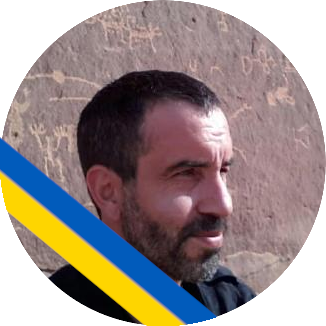
\includegraphics[width=3.5cm, right]{id}}

\includegraphics[scale=0.005]{phone} \quad (+0034) 693 726 091 \\

\includegraphics[scale=0.025]{gmail} \quad \href{mailto:thomashuet7@gmail.com}{thomashuet7@gmail.com} \\

\includegraphics[scale=0.01]{orcid} \quad \href{https://orcid.org/0000-0002-1112-6122}{0000-0002-1112-6122} \\

\includegraphics[scale=0.01]{github} \quad \href{https://github.com/zoometh/thomashuet.github.io/blob/main/README.md}{zoometh} \\

\includegraphics[scale=0.025]{gscholar} \quad \href{https://scholar.google.fr/citations?user=2hKEVaIAAAAJ}{2hKEVaIAAAAJ} \\

\includegraphics[scale=0.05]{rgate} \quad \href{https://www.researchgate.net/profile/Thomas\_Huet2}{Thomas\_Huet2} \\
\\

\begin{adjustwidth}{50pt}{50pt}
\begin{center}
\large{\textbf{Curriculum Vitae}}\\
\large{Prehistory, Computational Archaeology (programming languages, GIS databases), scientific writing} 
\end{center}
\end{adjustwidth}

\tableofcontents

\section{FIELDWORK EXPERIENCE (2012-)}

\textbf{2020 }Survey of the medieval engravings of Saur\'i (Catalonia, Spain), 2${}^{nd\ }$campaign, Universitat Aut\'{o}noma de Barcelona (UAB), Spain, 19 October --- 24 October.
\smallbreak
\textbf{2019-20 }Field engineering management of the oasis survey of Al-'Ula (oasis of Al-'Ula, Saudi-Arabia), Archa\"{i}os, AFALULA-RCU.
\smallbreak
\textbf{2019 }Survey of the medieval engravings of Sauri (Catalonia, Spain), 1${}^{st\ }$campaign, Universitat Aut\'{o}noma de Barcelona (UAB), Spain, 15 September --- 15 October.
\smallbreak
\textbf{2019 }Excavations of Nahal Efe (Negev Desert, Israel), Israel Antiquities Authorities (IAA) / Instituci\'{o}n Mil\'{a} y Fontanals - Consejo Superior de Investigaciones Cient\'{i}ficas (IMF-CSIC), resp. J.K. Sharvit and F. Borrell, Ein Tamar, 29 April --- 25 may.
\smallbreak
\textbf{2014 }Inventory/Study of the archaeological artefacts of Ciari's shelter conserved in: Museo Civico -- Cuneo; Superintendencia - Turin, in collaboration with N. Bianchi (Institute of Human Paleontology) and D. Binder (CEPAM-CNRS), 20-21 October.
\smallbreak
\textbf{---  }Paleoenvironmental coring, mont Bego archaeological site (Alpes-Maritimes, France), UMR 6249, Laboratoire Chrono-Environnement, Lac des Grenouilles, dir. B. Vanni\'{e}re, 6 --- 9 October.
\smallbreak
\textbf{---  }Photogrammetry and topography, archaeological \textit{hypog\'{e}e} de Vert-la-Gravelle (Marne, France), dir. R. Martineau, UMR 6298, ARTeHis, 15 --- 30 August.
\smallbreak
\textbf{---  }Archaeological excavations, Ponteau-Gare archaeological settlement (Bouches-du-Rh\^{o}ne, France), dir. X. Margarit, SRA-PACA, 1 --- 15 July.\smallbreak
\textbf{2013 }Aerial\textbf{ }photogrammetry and topography of the medieval Church of Saint Colomban Monastery archaeological site, Haute-Sa\^{o}ne, UMR 6298, ARTeHis -- NUI Galway, dir. S. Bully and E. Marron, 6 --- 8 August.
\smallbreak
\textbf{2012 }Paleoenvironmental coring, mont Bego archaeological site, Lac Long Inf\'{e}rieur and Lac des Grenouilles (Alpes-Maritimes, France), UMR 6249, Laboratoire Chrono-Environnement, dir. M. Magny, 19 --- 25 August

\section{ACADEMIC \textit{\&} PROFESSIONAL POSITIONS (2014-)}

\textbf{2021 }Specialist Research Support Technician, Departament de Prehist\`oria, Universitat Aut\'{o}noma de Barcelona (UAB), Spain, 1 July --- 31 December.
\smallbreak
\textbf{2020 }Co-responsible of the survey of the medieval engravings of Sauri (Catalonia, Spain), 2${}^{nd\ }$campaign, Universitat Aut\'{o}noma de Barcelona (UAB), Spain, 19 October --- 24 October.
\smallbreak
\textbf{2019-20 }Researcher at Archa\"{i}os company, in charge of the database integration for the survey of Al-'Ula, Saudi-Arabia (Archa\"{i}os, AFALULA, RCU).
\smallbreak
\textbf{2019 }Co-responsible of the survey of the medieval engravings of Sauri (Catalonia, Spain), 1${}^{st\ }$campaign, Universitat Aut\'{o}noma de Barcelona (UAB), Spain, 15 September --- 15 October.
\smallbreak
\textbf{---  }Project designer for the creation of a technological hub in Emerging technologies for Humanities, UMR 8546 CNRS/PSL --- AOrOc, Paris, resp. K. Gruel. Project granted.
\smallbreak
\textbf{2018 }Research Associate (IR), UMR 7264 CEPAM---CNRS, Universit\'{e} Nice Sophia-Antipolis, project \textit{C\'{e}ramiques Imprim\'{e}es de M\'{e}diterran\'{e}e occidentale} (CIMO), resp. D. Binder, 1 May --- 30 August and 1 October --- 30 November.
\smallbreak
\textbf{---  }Research Associate (IR), UMR 5140, ASM-CNRS, Universit\'{e} Paul Val\'{e}ry Montpellier 3, project \textit{EpiSpat} (aka \textit{ArchaEpigraph}), LabEx ARCHIMEDE, resp. C. Pellecuer, 1 April --- 1 May and 1 --- 30 September.
\smallbreak
\textbf{2017-18 }Training, recording techniques of rock-art and engraved steles of South-West Iberic peninsula (\textit{Tecniques d'enregistrament de l'art rupestre de les esteles gravades del Sud-oest de la Peninsula ibèrica}), Grupo de investigaci\'{o}n "Arqueolog\'{i}a de las din\'{a}micas sociales", Instituci\'{o}n Mil\'{a} y Fontanals (IMF) - Consejo Superior de Investigaciones Cient\'{i}ficas (CSIC), Barcelone, resp. S. Valenzuela, 1 September 2017 --- 30 May 2018.
\smallbreak
\textbf{2017 }Development of the Information system (GIS, datatabase, topography and photogrammetry), grotte de Pertus II, Alpes-de-Haute-Provence, UMR 7264 CEPAM-CNRS, Universit\'{e} Nice Sophia-Antipolis and Ev\'{e}ha, resp. C. Lep\`{e}re, 7 --- 27 July.
\smallbreak
\textbf{2016 }Development of the information system (GIS, database, topography and photogrammetry) of Pertus II cave, Alpes-de-Haute-Provence, dir. C. Lep\`{e}re, 1 --- 15 August 2016.
\smallbreak
\textbf{2015-16 }Postdoctoral fellow, LabEx ARCHIMEDE, UMR 5140 ASM-CNRS and University Paul-Val\'{e}ry, Montpellier. Project: 'Study of Final Bronze Age figurative ceramic decorations in South France and Northeastern Spain', 1 October 2015 --- 30 September 2016.
\smallbreak
\textbf{2015 }Auditor in the research seminar "Regards crois\'{e}s sur la notion de paysage", lector~: S.~Robert, EHESS, March --- June.\textbf{}
\smallbreak
\textbf{2014 }Research\textbf{ }Associate (IR), project \textit{Archaepigraph} project, UMR 6249 Chrono-Environnement, Universit\'{e} de Franche-Comt\'{e}, dir. M.-J. Ouriachi and L. Nuninger, 1 September --- 30 October.
\smallbreak
\textbf{2013-14  }Research Assistant (IE), USR CNRS -- UB 3516, GeoBFC platform, MSH de Dijon, Universit\'{e} de Bourgogne, project OH-FET (Historical Object, Function, Space, Time), dir. L. Saligny, 1 June --- 31 May.

\section{EDUCATION (2003-)}

\textbf{2013 }PhD prize for publication. CASDEN -- Banque Populaire (UFR LSH, Universit\'{e} Nice Sophia-Antipolis).
\smallbreak
\textbf{2006-12 }PhD History and Archaeology, first level of distinction (''mention tr\'{e}s honorable avec les f\'{e}licitations du jury''). PhD title: ''Organisation spatiale et s\'{e}riation des gravures piquet\'{e}es du mont Bego'', Universit\'{e} Nice Sophia-Antipolis, UMR 7264 CEPAM-CNRS.
\smallbreak
\textbf{2005-6 }Master Research ('mention bien') "Sciences de l'Homme et de la Soci\'{e}t\'{e} Histoire et Arch\'{e}ologie", mention~: "Sciences des Mondes Pr\'{e}historiques, Antiques et M\'{e}di\'{e}vaux", Universit\'{e} Nice Sophia-Antipolis, CEPAM-CNRS UMR 7264.
\smallbreak
\textbf{2004-5 }DUT (University Diploma of Technology) Informatics Engineering (''mention assez bien''), Conservatoire National des Arts et M\'{e}tiers, Paris.
\smallbreak
\textbf{2003 } Topography diploma, Universitad de Ingenier\'{i}a, Lima, Peru.

\section{PUBLICATIONS (2014-)}

\begin{center}------------ Books ------------ \end{center}

$\cdot$ \textbf{Huet T., 2017}, \textit{Les gravures piquet\'{e}es du mont Bego (Alpes-Maritimes). Organisation spatiale et s\'{e}riation (6e -- 2e mill\'{e}naire av. J.-C.)}, M\'{e}moire de la Soci\'{e}t\'{e} Pr\'{e}historique Fran\c{c}aise (SPF) 63, 166 p. \href{http://www.prehistoire.org/shop_515-40342-0-0/m63-2017-les-gravures-piquetees-du-mont-bego-alpes-maritimes-organisation-spatiale-et-seriation-vie-iie-millenaire-av.-j.-c.-t.-huet.html}{url} 
\bigbreak
\begin{center}------------ Book chapters ------------\end{center}
\smallbreak
$\cdot$ Alexander C., Maretta A., \textbf{Huet T.} and C. Chippindale, \textbf{2021}, Rules of ordering and grouping in the 'pitoti', the later prehistoric rock-engravings of Valcamonica (BS), Italy: from solitary figures through clusters, graphic groups, and scenes to narrative, in I. Davidson and A. Nowell (eds), \textit{Making scenes: global perspectives on scenes in rock art}, London: Berghahn Books. \href{https://www.berghahnbooks.com/title/DavidsonMaking}{url}
\smallbreak
$\cdot$ \textbf{Huet T., 2018}, Une revue de l'iconographie du d\'{e}but du N\'{e}olithique \'{a} la fin de l'\^{a}ge du Bronze (ca. 5700-750 av. J.-C.) en France, \textit{in} Guilaine J. et D. Garcia (dir.), \textit{La Protohistoire de la France}, ed. Hermann, Paris, p. 221-249. \href{https://hal.archives-ouvertes.fr/hal-01983284}{hal-01983284}
\bigbreak
\begin{center}------------ Indexed journals ------------\end{center}
\smallbreak
$\cdot$ \textbf{Huet T.}, Pozo J. M., Alexander C., \textbf{2021}, Analysis of Prehistoric Iconography with the R package iconr, \textit{JOSS}, \href{https://joss.theoj.org/papers/10.21105/joss.03191}{10.21105/joss.03191}
\smallbreak
$\cdot$ Nieto-Espinet A., \textbf{Huet T.}, Trentacoste A., Guimaraes S., Orengo H. and Valenzuela-Lamas S., \textbf{2021}, Resilience and livestock adaptations to demographic growth and technological change: A diachronic perspective from the Late Bronze Age to Late Antiquity in NE Iberia, \textit{PlosONE}, \href{https://doi.org/10.1371/journal.pone.0246201}{10.1371/journal.pone.0246201}
\smallbreak
$\cdot$ Iba\~{n}ez J.J., Mu\~{n}iz J., \textbf{Huet T.}, Borrell Terra F.,  Santana Y., Teira Mayolini L.C. and R. Rosillo, \textbf{2020}, Flint Figurines in the Early Neolithic site of Kharaysin (Early 8th Millennium BC, Jordan), \textit{Antiquity Journal, 94, 376} p. 880-899, \href{https://doi.org/10.15184/aqy.2020.78}{10.15184/aqy.2020.78}
\smallbreak
$\cdot$ Cicolani V. and \textbf{T. Huet, 2019}, Essai de mod\'{e}lisation des \'{e}changes et des r\'{e}seaux de circulation dans les Alpes centrales au premier \^{a}ge du Fer, \textit{in} "La conqu\^{e}te de la montagne : des premi\'{e}res occupations humaines \'{a} l'anthropisation du milieu", CTHS \'{e}ditions, \href{https://halshs.archives-ouvertes.fr/halshs-02314978/document}{halshs-02314978}
\smallbreak
$\cdot$ \textbf{Huet T.,} \textbf{2018}, Geometric Graphs to Study Ceramic Decoration\textit{, in} M. Matsumoto and  E. Uleberg (eds), Exploring Oceans of Data, \textit{Proceedings of the 44${}^{nd\ }$Conference on Computer Applications and quantitative Methods in Archaeology} (CAA 2016), Oxford : Archaeopress Archaeology, 311-323.\href{https://hal.archives-ouvertes.fr/hal-02913656}{hal-02913656}
\smallbreak
$\cdot$ \textbf{Huet T., 2016}, New perspectives on the chronology and the meaning of Mont Bego's rock-art (Alpes-Maritimes, France), \textit{Cambridge Archaeological Journal} 41, 1-23, \href{https://doi.org/10.1017/s0959774316000524}{10.1017/s0959774316000524}
\smallbreak
$\cdot$ \textbf{Huet T.} and N. Bianchi, \textbf{2016}, Reticolati, pelli e mappe topografiche, lo stato della ricerca al monte Bego, \textit{Bollettino del Centro Camuno di Studi Preistorici} 41, 31-43. \href{http://www.ccsp.it/web/infoccsp/bcsp/bcsp41_preview.pdf}{url}
\smallbreak
$\cdot$ \textbf{Huet T.} and N. Bianchi, \textbf{2016}, A study of the Roche de l'Autel's pecked engravings, Les Merveilles sector, Mont Bego area (Alpes-Maritimes, France), \textit{Journal of Archaeological Sciences: Reports} 5, 105-118, doi: \href{https://doi.org/10.1016/j.jasrep.2015.11.006}{10.1016/j.jasrep.2015.11.006}
\smallbreak
$\cdot$ \textbf{Huet T., 2016}, S\'{e}riation des gravures piquet\'{e}es du mont Bego, \textit{Archeologia e Calcolatori} 27, 65-83. \href{https://doi.org/10.19282/AC.27.2016.02}{10.19282/AC.27.2016.02}
\smallbreak
$\cdot$ \textbf{Huet T.,} \textbf{2015}, Le incisioni a martellina del monte Bego: approcci geografici e quantitativi, \textit{Archeologia Postmedievale} 17, 329-338. \href{https://www.insegnadelgiglio.it/wp-content/uploads/2015/01/APM_17_libro-anteprima.pdf}{url}
\smallbreak
$\cdot$ Saligny L., Granjon L., \textbf{Huet T.}, Simon G., Rodier X. and B. Lefebvre \textbf{2015}, OH\_FET: A Computer Application for Analysing Urban Dynamics Over Long Time Spans, in\textit{ Proceedings of the 42${}^{nd\ }$Conference on Computer Applications and quantitative Methods in Archaeology} (CAA 2014), eds\textit{. }Giligny F., Djindjian F., Costa L., Moscati P. et S. Robert, Oxford : Archaeopress Archaeology, 381-392.\href{https://hal.archives-ouvertes.fr/halshs-01146871}{halshs-01146871}
\smallbreak
$\cdot$ \textbf{Huet T.} and C. Alexander, \textbf{2015}, M\'{e}thodes informatiques pour l'\'{e}tude des gravures rupestres~: les exemples du Valcamonica (Italie) et du mont Bego (France), in \textit{Recherches sur l'\^{a}ge du Bronze. Nouvelles approches et perspectives. Actes de la journ\'{e}e d'\'{e}tude de l'APRAB, Bulletin de l'APRAB, suppl. 1}, 15-29.
\smallbreak
$\cdot$ Ouriachi M.-J., Favory F., Garmy P., Ouzoulias P., Pasqualini A., Christol M., \textbf{Huet T}., Nuninger L., Bertoncello F., H\"{a}ussler R.. \textbf{2014}, ArchaEpigraph : l'\'{e}pigraphie spatiale au service de l'\'{e}tude des dynamiques des territoires, in \textit{Revue arch\'{e}ologique de Narbonnaise}, tome 47, pp. 35-49.\href{https://www.persee.fr/doc/ran_0557-7705_2014_num_47_1_1897}{url}
\smallbreak
$\cdot$ \textbf{Huet T.,} \textbf{2014}, Use of quantitative methods to study an Alpine rock art site: the Mont Bego region, in \textit{Proceedings of the 40${}^{th}$ Conference on Computer Applications and quantitative Methods in Archaeology} (CAA 2012), eds. Earl G., Sly T., Chrysanthi A., Murrieta Flores P., Papadopoulos C., Romanowska I. et D. Wheatley, Southampton, UK, 26-30 March 2012, Amsterdam : Pallas Publications, , 584-591.
\smallbreak
$\cdot$ \textbf{Huet T.,} \textbf{2014}, Organisation spatiale et s\'{e}riation des gravures piquet\'{e}es du mont Bego~-- R\'{e}sum\'{e} de th\'{e}se, \textit{Bulletin de la Soci\'{e}t\'{e} Pr\'{e}historique Fran\c{c}aise} 110, 146-148.\href{https://www.persee.fr/doc/bspf_0249-7638_2013_num_110_1_14242}{url}

\subsection*{Scientific Conferences \textit{\&} Seminars (2014-)}
\begin{center}(\textbf{i}) international audience {\textbar} (\textbf{n}) national audience \end{center}
\smallbreak
\begin{center}------------ Organisation ------------\end{center}
\smallbreak
\textbf{2016 }S\'{e}minaire d'\'{e}quipe ASM-CNRS (UMR 5140), \'{e}quipe Soci\'{e}t\'{e}s de la Pr\'{e}histoire et de la Protohistoire, Analyser et interpr\'{e}ter les d\'{e}cors des c\'{e}ramiques pr\'{e}- et protohistoriques. Approches crois\'{e}es, co-organis\'{e} avec T. Lachenal et K. Peche-Quichilini, Universit\'{e} Paul-Val\'{e}ry, Montpellier, 27 May. (\textbf{n})
\smallbreak
\textbf{2014 }Session n$\mathrm{{}^\circ}$ 20 :\textit{ "(Re)building past networks: archaeological science, GIS and network analysis"}, co-organised with C. Alexander, S. Robert, E. Mermet, 42${}^{th}$ international congress of the \textit{Computer Applications and Quantitative Methods in Archaeology} (CAA 2014), Universit\'{e} Sorbonne, France, 22-25 April. (\textbf{i})
\bigbreak
\begin{center}------------ Communications ------------\end{center}
\smallbreak
\textbf{2021 }"Managing and analysing pictorial documentation with GIS and graphs", co-presented with C. Alexander and J. Pozo, International congress of the \textit{Computer Applications and Quantitative Methods in Archaeology} (CAA 2021), Cyprus University of Technology, Cyprus, 14 March-18 June \href{https://youtu.be/tUhHhzGSgbk?t=4950}{
\includegraphics[scale=0.2]{icon_youtube}} \textbf{(i)}
\smallbreak
\textbf{---  }"Between Celtic, Italic and Etruscan worlds. Re-thinking Boundaries and Models of Interaction across the Alps", co-presented with V. Cicolani and L. Zamboni, Adaptation and Creativity along Border Zones, Charles University, Prague, 31 May - 3 June \textbf{(i)}
\smallbreak
\textbf{---  }"Paisatges de conflicte i de poder. Els gravats medievals del Sol\`{a} de Saur\`{i} (Pallars Sobir\`{a})", co-presented with E. Gassiot Ballb\`{e} and O. Aug\'{e} Mart\'{i}nez, Tribuna d'Arqueologia, Barcelona, 21 April \href{https://www.youtube.com/watch?v=4b7gLw4NV_E}{
\includegraphics[scale=0.2]{icon_youtube}} \textbf{(n)}
\smallbreak
\textbf{2019 }"Diacronia delle incisioni rupestri preistoriche e protostoriche della regione del monte Bego (Tenda, Alpi Marittime, Francia)", co-presented with J. Masson Mourey J. and N. Bianchi, LIV Riunione scientifica, Archeologia del cambiamento. Modelli, processi, adattamenti nella Preistoria e Protostoria, Roma, 23-26 October. \textbf{(i)}
\smallbreak
\textbf{---  }"The North-western Impressed Wares: a chrono-cultural overview", co-presented with D. Binder, L. Angeli, L. Gomart, R. Maggi, C. Manen, I.M. Muntoni, E. Natali, C. Panelli, G. Radi, F. Radina, C. Tozzi, S. Tusa, 1st conference on the Early Neolithic of Europe (ENE2019), Barcelona, 6-9 November. \textbf{(i)}
\smallbreak
\textbf{---  }"L'Impresso-cardial du nord-ouest et ses rapports avec la "zone-source" : une synth\'{e}se chrono-culturelle", co-presented with D. Binder, L. Angeli, L. Gomart, R. Maggi, C. Manen, I. Maria Muntoni, E. Natali, C. Panelli, G. Radi, F. Radina, C. Tozzi, S. Tusa, S\'{e}ance de la Soci\'{e}t\'{e} Pr\'{e}historique Fran\c{c}aise, Nice, 18-20 March.\textbf{ (i)}
\smallbreak
\textbf{---  }"Territorialit\'{e}, mobilit\'{e}, interactions : apports crois\'{e}s des sous-syst\'{e}mes lithiques et c\'{e}ramiques", co-presented with D. Binder, C. De Stefanis, P. Fernandes, B. Gratuze, R. Maggi, C. Tozzi, S\'{e}ance de la Soci\'{e}t\'{e} Pr\'{e}historique Fran\c{c}aise, Nice, 18 - 20 March.\textbf{ (i)}
\smallbreak
\textbf{2018 }"Pastoral graffiti and ''protohistoric'' engravings in Mont Bego region: a study of marking practices over long time spans", co-presented with N. Magnardi, 20${}^{e}$ international rock-art congress organisation (ifrao), Darfo Boario Terme, 29 August-2 September.\textbf{ (i)}
\smallbreak
\textbf{2017 }"Las representaciones iconogr\'{a}ficas en Francia del Neol\'{i}tico antiguo a la fin del Edad del Bronce (5700-750 BC)", SEMINARIOS Grupo de investigaci\'{o}n "Arqueolog\'{i}a de las din\'{a}micas sociales", Instituci\'{o}n Mil\'{a} y Fontanals (IMF) - Consejo Superior de Investigaciones Cient\'{i}ficas (CSIC), Barcelone, 12 December. (\textbf{n})
\smallbreak
\textbf{---  } "Interactions culturelles au Premier \^{a}ge du Fer dans les Alpes occidentales : essai de mod\'{e}lisation des \'{e}changes par la th\'{e}orie des r\'{e}seaux~", co-presented with V. Cicolani, 142${}^{e}$ congr\'{e}s du \textit{Comit\'{e} des Travaux Historiques et Scientifiques} (cths), Pau, 24-29 April.\textbf{ (n)}
\smallbreak
\textbf{2016 }"Geometrical and planar graphs in ancient iconography studies, a heuristic tool", 44${}^{th}$ international congress of the \textit{Computer Applications and Quantitative Methods in Archaeology} (CAA 2016), University of Oslo, Sweden, 29 March-2 April. (\textbf{i})
\smallbreak
\textbf{---  }"L'\'{e}tude des d\'{e}cors c\'{e}ramiques figuratifs du Mailhac I et des d\'{e}cors apparent\'{e}s (Bronze final IIIb). Contextes, m\'{e}thodes et premiers r\'{e}sultats" journ\'{e}e th\'{e}matique Images et imaginaire \'{a} l'\^{A}ge du bronze en Europe, \textit{Association pour la Promotion de la Recherche sur l'\^{A}ge du Bronze} (APRAB), Mus\'{e}e des Antiquit\'{e}s Nationales, Saint-Germain-en-Laye, 4 March. (\textbf{n})
\smallbreak
\textbf{2015 }"Les gravures rupestres n\'{e}olithiques du mont Bego (Alpes-Maritimes) : identifications, comparaisons et significations suppos\'{e}es", \textit{L'art n\'{e}olithique du Proche-Orient \'{a} l'Europe : nouvelles, approches th\'{e}oriques et m\'{e}thodologiques}, round table of the \textit{Association pour le D\'{e}veloppement des Rencontres et des Echanges Universitaires et Culturels} (adreuc), Notre Dame de l'Abbaye, Carcassonne, 5 November. (\textbf{n})
\smallbreak
\textbf{---  }"Familles aristocratiques dans la cit\'{e} antique de N\^{i}mes : un exemple de mise en r\'{e}seaux des individus par les monuments \'{e}pigraphiques (Ier si\'{e}cle av. notre \'{e}re -- IIIe si\'{e}cle)" co-pr\'{e}sent\'{e}e avec M.-J. Ouriachi, 140${}^{th}$ congress of the \textit{Comit\'{e} des Travaux Historiques et Scientifiques} (cths), Reims, 27 April-2 May. (\textbf{n})
\smallbreak
\textbf{2014 }"Ancient pastoral paths in mount Bego rock art area" Session \textit{(Re)building past networks: archaeological science}, GIS and network analysis, 42${}^{th}$ international congress of the \textit{Computer Applications and Quantitative Methods in Archaeology} (CAA 2014), Universit\'{e} Sorbonne, France, 22-25 April. (\textbf{i})\textbf{}
\smallbreak
\textbf{---  }"OH-FET : a computer application to compare urban dynamics over long time spans (longue dur\'{e}e)", Session n$\mathrm{{}^\circ}$ 18, co-presented with L. Saligny, L. Granjon, B. Lefebvre, G. Simon, X. Rodier, 42${}^{th}$ international congress of the \textit{Computer Applications and Quantitative Methods in Archaeology} (CAA 2014), Universit\'{e} Sorbonne, France, 22-25 April. (\textbf{i})
\smallbreak
\textbf{---  }"M\'{e}thodes informatiques en art rupestre. Etudes de cas : le Valcamonica et le mont Bego", co-presented with C. Alexander, thematic day \textit{Recherches sur l'\^{A}ge du Bronze }of the\textit{ Association pour la Promotion de la Recherche sur l'\^{A}ge du Bronze }(APRAB), Mus\'{e}e des Antiquit\'{e}s Nationales, Saint-Germain-en-Laye, 28 February. (\textbf{n})

\section{ACADEMIC \textit{\&} RESEARCH PROGRAMS (2014-)}

\subsection*{Teachings}

\textbf{2017 }"Introduction to Geographic Information Systems: QGIS", \textit{Grupo de Arqueologia de las Din\'{a}micas Sociale}s, Consejo Superior de Investigaciones Cientificas, Instituci\'{o}n Mil\'{a} i Fontanals (CSIC-IMF), 14-16 December (9 heures).
\smallbreak
\textbf{---  }"Les repr\'{e}sentations d'attelages \'{a} l'\^{a}ge du Bronze (Espagne, France, Italie), dans le cadre du \textit{S\'{e}minaire de formation doctorale du r\'{e}seau interdisciplinaire AniMed}, University seminar, Universit\'{e} Paul-Val\'{e}ry, 26 January (1 hour).
\smallbreak
\textbf{2016 }"M\'{e}thodes quantitatives en arch\'{e}ologie. L'approche processuelle : concepts, outils et cas d'\'{e}tude" Master 2 Arch\'{e}ologie, Sciences pour l'Arch\'{e}ologie, ASM-UMR 5140, University seminar, Universit\'{e} Paul-Val\'{e}ry, 5 December (4 hours).
\smallbreak
\textbf{2015 }"L'apparition des d\'{e}cors figuratifs du Mailhac I et des groupes apparent\'{e}s dans une Europe continentale largement aniconique (Bronze final IIIb, 950-750 av. J.-C.) : contextes, hypoth\'{e}ses et m\'{e}thodes" Master 1 Recherche, Protohistoire m\'{e}diterran\'{e}enne, ACTE -- UE 3-6, University seminar, Universit\'{e} de Bourgogne, 24 November (1 hour).
\smallbreak
\textbf{---  }"L'apport du SIG \'{a} l'\'{e}tude de l'art rupestre du Mont Bego (Alpes-Maritimes)" Master 2 Recherche et Professionnel, Arch\'{e}ologie des Soci\'{e}t\'{e}s et Territoires en France M\'{e}tropolitaine, M\'{e}thodes et approches nouvelles, LARA, CReAAH-UMR 6566, University seminar, Universit\'{e} de Nantes, Universit\'{e} de Rennes, 4 November (1 hour).
\smallbreak
\textbf{---  }"Les m\'{e}thodes quantitatives en arch\'{e}ologie : de la \textit{New Archaeology} au \textit{Project Mosul}" Master 2 Recherche et Professionnel, Arch\'{e}ologie des Soci\'{e}t\'{e}s et Territoires en France M\'{e}tropolitaine, S\'{e}minaire sp\'{e}cialis\'{e} : "M\'{e}thodes et approches nouvelles", LARA, CReAAH-UMR 6566, University seminar, Universit\'{e} de Nantes, Universit\'{e} de Rennes, 16 October (1 hour).
\smallbreak
\textbf{---  }"Data Paths", University workshop, Z\'{a}pado\v{c}esk\'{a} Univerzita (\textit{University of West Bohemia}), Pilsen, Czech Republic, 12 March, (1 hour).

\subsection*{Research Programs}

\subsubsection*{Academic committees}

- Member of the PhD steering committee (2015-2020) of: Francis Bordas, University Toulouse 2, Doctoral section TESC, UMR TRACES, PhD title: "Les d\'{e}p\^{o}ts d'objets m\'{e}talliques au Bronze final 3 dans l'espace atlantique fran\c{c}ais (950-800 av J.-C.) : modalit\'{e}s de constitution des d\'{e}p\^{o}ts fran\c{c}ais de l'\'{e}tape de l'\'{e}p\'{e}e du type en langue de carpe."
\smallbreak
- Tutor of the Master 2  steering committee (2018-2019) of: Marco Padovan, University Toulouse 2, "Formation aux outils de traitement 3D" dans le cadre du Master 2 de, Universit\'{a} degli studi di \textit{Ferrara} (Italia), Master 2 title: "The Fabric of the Baume de Monthiver"

\subsubsection*{Journal committees}

-  Member of the editorial board of the \textit{Pr\'{e}histoires M\'{e}diterran\'{e}ennes} journal (2021 --- ...)\\ 
-  Reviewer for the \textit{Bulletin de la Soci\'{e}t\'{e} Pr\'{e}historique Fran\c{c}aise} journal (2020 --- ...)\\  
-  Reviewer for the \textit{M@ppemonde} journal (2019 --- ...)\\ 
-  Reviewer for the \textit{CAA Review College} (2014 --- ...)\\ 

\subsubsection*{Collective research projects}

-  Member of the \href{https://sslarch.github.io/}{SIG-SSLA} Special Interest Group on Scientific Scripting Languages in Archaeology  (2020 --- ...)\\ 
-  Member of the \href{https://arqueologiademuntanya.wordpress.com/}{Grup d'Arqueologia de l'Alta Muntanya (GAAM)} (UAB, CSIC) (2021 --- ...)\\ 
-  Member of the \href{https://redneonet.com/}{NeoNet} collective research project, resp. J. Gibaja, M. Cubas (2020 --- ...)\\ 
-  Former member of the \textit{Corpus des signes grav\'{e}s n\'{e}olithiques} collective research project, resp. S. Cassen\\  
-  Former member of the \textit{Information Spatiale et Arch\'{e}ologie} network (ISA)\\ 
-  Former member of the "~Faire Science avec l'Incertitude en SHS~" work group, MSH Nice\\ 
-  Former member of the \textit{Evolutions, transferts, inter-culturalit\'{e}s dans l'arc liguro-proven\c{c}al : Mati\'{e}res premi\'{e}res, productions et usages, du Pal\'{e}olithique sup\'{e}rieur \'{a} l'\^{a}ge du Bronze ancien} (ETICALP) collective research project (PCR), resp. D. Binder  


\section{IT RELEASES \textit{\&} INFORMATIC TOOLS}

\subsection*{IT releases}

\subsubsection*{Softwares and Packages}

\textbf{2021 }\href{https://cran.r-project.org/web/packages/iconr/index.html}{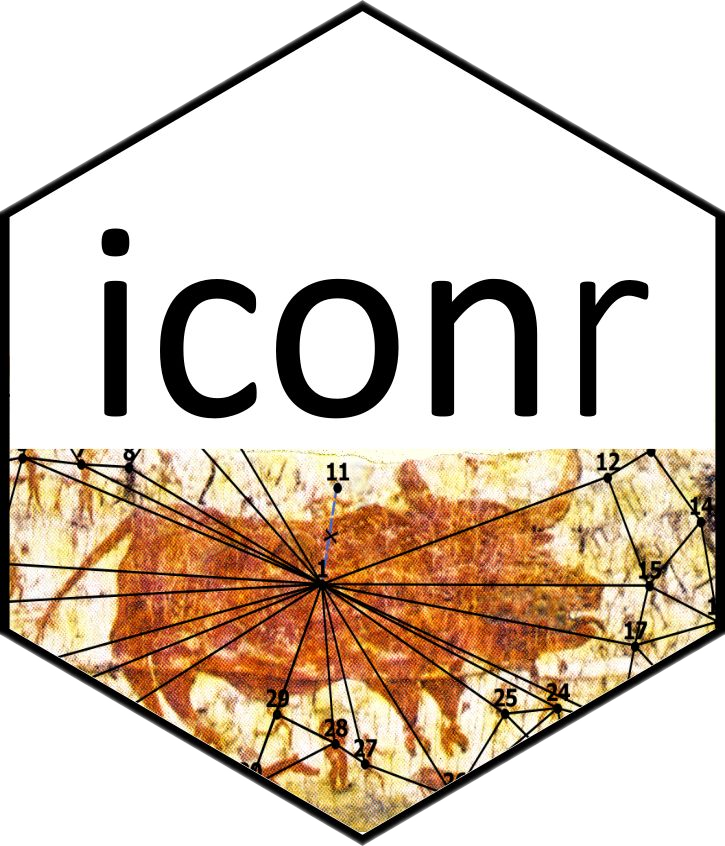
\includegraphics[scale=0.035]{iconr_logo}} \textsf{R} package, v. 0.1.0 CRAN stable release, with Jose Pozo and Craig Alexander.
\smallbreak
\textbf{2014 }\href{https://www.oxbowbooks.com/dbbc/caa2014-21st-century-archaeology.html/}{OH-FET application v.1}, a \textsf{Python} app to compare urban dynamics over long time spans (with Ludovic Granjon and Laure Saligny, MSH de l'Universit\'{e} de Bourgogne).

\subsubsection*{Web applications}

\textbf{2018 }\href{https://epispat.shinyapps.io/analyses_mult_5/}{EpiSpat application} \textsf{RShiny} interactive web application for multifactorial on-the-fly clustering of Roman epigraphic stelae.
\smallbreak
\textbf{2020 }\href{https://neolithic.shinyapps.io/neonet2/}{
\includegraphics[scale=0.04]{neonet}} \textsf{RShiny} interactive web application for selecting, calibrating, summing and plotting on-the-fly radiocarbon dates. EUROEVOL\_R parses the \href{http://discovery.ucl.ac.uk/1469811/}{EUROEVOL database} (Institute of Archaeology, UCL).

\subsubsection*{Web docs}

\textbf{2021 }\href{https://zoometh.github.io/rockart/}{\textbf{Rock-art}}, \textsf{R} + \textsf{Markdown} document. Multi-paradigm and multi-scalar management of rock-art data with open-source softwares (\textsf{3DHOP}, \textsf{Leaflet}, \textsf{GitHub}, etc.)
\smallbreak
\textbf{2021 }\href{https://zoometh.github.io/aDNA/}{\textbf{Gene-culture} coevolution (GC-coev)}, \textsf{R} + \textsf{Markdown} document. Reuse of existing aDNA data and cross-analysis methods with radiocarbon dates and culture data
\smallbreak
\textbf{2021 }\href{https://zoometh.github.io/C14/neonet/}{
\includegraphics[scale=0.04]{neonet}} \textsf{R} + \textsf{Markdown} tutorial document. 
\smallbreak
\textbf{2021 }\href{https://neolithic.shinyapps.io/AbsoluteDating/}{Absolute dating}, \textsf{R} + \textsf{Markdown} document. Web applications and databases review for archaeological radiocarbon and dendrochronological dates.
\smallbreak
\textbf{2020 }\href{https://zoometh.github.io/golasecca/}{Golasecca-net}, \textsf{R} + \textsf{Markdown} document for archaeological data visualisation (maps, charts, spatial networks) of movable goods (personal ornements, imported/prestige goods) \href{https://doi.org/10.5281/zenodo.4315328}{10.5281/zenodo.4315328}.
% \includegraphics{{mds}}

\subsection*{Informatic tools}
\begin{center}(\textbf{\textsuperscript{-}}) notions \end{center}
\smallbreak

\subsubsection*{OS {\textbar} Programming languages}

Windows, Linux\textsuperscript{-} \textbf{{\textbar}} \textsf{R}, \textsf{Python}, \textsf{JavaScript\textsuperscript{-}}, SQL, markup languages (JSON, XML, HTML, CSS, etc.)

\subsubsection*{Servers  {\textbar} Databases development} 

Apache\textsuperscript{-} \textbf{{\textbar}} PostgreSQL/GIS, FileMaker, SpatiaLite, Access, NoSQL databases\textsuperscript{-}

\subsubsection*{Software development} 

\textsf{R} package with continuous integration (GitHub, Travis-CI), \textsf{Python} to executable (.exe) with Pyinstaller

\subsubsection*{Web authoring \& Data driven documents {\textbar} Desktop publishing {\textbar} Web platforms}

\textsf{Sweave}, \textsf{Rmarkdown}, \textsf{RShiny}, \textsf{Plotly}, \textsf{IPython\textsuperscript{-}}, \textbf{{\textbar}}  \LaTeX, Windows Office \textbf{{\textbar}} RPubs, Zenodo

\subsubsection*{Images 2D and 3D}

\paragraph*{Infography {\textbar} Images management \& metadata}

ImageMagick, ImageJ, and current graphic softwares (Gimp, Photoshop, Inkscape, Illustrator,etc.) {\textbar} ExifTool , XnView, Piwigo, etc.

\paragraph*{Photogrammetry/RTI {\textbar} 3D creation {\textbar} Web 3D}

PhotoScan,  MicMac\textsuperscript{-}, RTIBuilder\textsuperscript{-} {\textbar} MeshLab, CloudCompare, Blender\textsuperscript{-} \textbf{{\textbar}} WebGL, 3DHOP, Potree\textsuperscript{-}

\subsubsection*{Geographical Information Systems (GIS) {\textbar} GeoCMS \& Geoweb services {\textbar} Geopositionning and topography}

QGIS, ArcGIS {\textbar} \textsf{Leaflet}, \textsf{OpenLayers\textsuperscript{-}}, WMS, WFS, WCS, etc. {\textbar} Differential GPS, Total Station, Theodolite

\subsubsection*{Agent-based modeling (ABM)}

NetLogo\textsuperscript{-}, \textsf{RNetLogo\textsuperscript{-}}

\section*{TRAINING COURSES ATTENDED}

\subsection*{Statistics }

\textbf{2014 }"\textsf{R} application", training of the \textit{ElementR} group, UMR 8504 G\'{e}ographie-cit\'{e}s, MSH de l'Universit\'{e} de Bourgogne (Dijon, France) 27-28 January.
\smallbreak
\textbf{2010 }"Describe and analyse multifactorial data", Permanent training of the CNRS Delegation C\^{o}te d'Azur (Sophia-Antipolis, France), 7-9 September.
\smallbreak
\textbf{---  }"Decide and predict with multifactorial data: discriminant analysis and regressions", Permanent training of the CNRS D\'{e}l\'{e}gation C\^{o}te d'Azur (Sophia-Antipolis, France), 16-18 June.
\smallbreak
\textbf{2009 }"Statistical processing of small samples", Permanent training of the CNRS Delegation C\^{o}te d'Azur (Sophia-Antipolis, France), 14-16 October.
\smallbreak
\textbf{---  }"Introduction to standard statistics", Permanent training of the CNRS Delegation C\^{o}te d'Azur (Sophia-Antipolis, France), 16-18 September.
\textbf{---  }"Statistical processing of design of experiments: analysis of variance", Permanent training of the CNRS Delegation C\^{o}te d'Azur (Sophia-Antipolis, France), 16-18 June.
\smallbreak

\subsection*{Network analysis}

\textbf{2018 }"MOSAIC${}^{NET\ }$2018: Networks in Archaeological Research", International Summer School at~Bibracte, Ecole Europ\'{e}enne de Protohistoire (Glux-en-Glenne, France), 8-13 October.

\subsection*{Agent-based modeling}

\textbf{2016 }"Agent-based modelling for archaeologists", workshop in parallel of the \textit{Computer Applications and Quantitative Methods in Archaeology} (CAA 2016) international colloquium (Oslo, Sweden), 28-29 March.

\subsection*{3D / Photogrammetry}

\textbf{2016 }"\textit{CloudCompare} - manipulation of 3D~clouds", workshop in parallel of the \textit{Journ\'{e}es informatique et arch\'{e}ologies de Paris} (jiap), Institut d'Art et d'Arch\'{e}ologie (Paris, France), 8 June.
\smallbreak
\textbf{---  }"\textit{MeshLab }- manipulation of 3D\textit{ }meshes", workshop in parallel of the \textit{Journ\'{e}es informatique et arch\'{e}ologies de Paris} (jiap), Institut d'Art et d'Arch\'{e}ologie (Paris, France), 7 June.
\smallbreak
\textbf{2013 }"Aerial photography by kite and helium balloon: shot, georeferencing and photogrammetry", CNRS Formations entreprises (Al\'{e}s, Berrias et Casteljau, France), 28-30 May.

\subsection*{Image / Shape analysis}

\textbf{2013 }"Detection of structures and spatio-morphological dynamics by image analyses: morpho-mathematics", training organised by ISA network, UMR 7264 CEPAM-CNRS and UMR 7300 ESPACE (Nice, France), 18-21 March.
\smallbreak
\textbf{---  }"ImageJ", Permanent training of the CNRS Delegation C\^{o}te d'Azur (Sophia-Antipolis, France), 11-13 February.

\subsection*{Archaeology}

\textbf{2017-18 } "Record and wear analysis of engraving technics", training at the IMF-CSIC (Barcelona, Spain), 1 September - 30 May.
\smallbreak
\textbf{2010 } "Traceology of pre- and protohistorical stone tools", UMR 7264 CEPAM-CNRS, Universit\'{e} Nice Sophia-Antipolis (Nice, France), 4-15 October.
\smallbreak
\textbf{2008 } "Statement of carvings in Valcamonica archaeological site", training of the Archaeoloical Cooperative ''Le Orme dell Uomo'' (Capo di Ponte, Italy), 1-15 July.
\smallbreak
\textbf{2007 } "Technics for the archaeological cast", Mus\'{e}e municipal d'arch\'{e}ologie de Cimiez (Nice, France), 3-15 December.

\section*{LANGUAGES \textit{\&} COMPLEMENTARY INFORMATIONS}

French: native \\
English, Spanish: good \\
Italian, Catalan: reading, listening \\
German: beginner \\
dialectal Arabic: notions \\

Driving licence (permis B), Diving level 1, Animation Capacity Diploma (BAFA)

\end{document}
